\chapter{Preliminaries and Related Work}\label{chapter:preliminaries_and_related_works}

Extracting information from large datasets is crucial to understanding their underlying structure. Data mining methods, such as clustering, extract patterns from a dataset by identifying the different coherent groups present in the data. Each group, or cluster, is a collection of similar data points which have small inter-point distances compared with distances to points in other clusters \parencite{bishop2006pattern}. In this chapter, we review clustering and how it can be used to identify objects in images.

This chapter is divided into two sections. In the first section, we consider data exploration through clustering and discuss a widely-used clustering algorithm. In the second section, we consider the more specific problem of extracting the different objects present in an image and review some of the different methods found in the literature.

\section{Clustering}

The problem of finding the globally optimal clustering result is an NP-hard problem \parencite{ayramo2006introduction}. One naive approach to obtaining the optimal clustering solution in a dataset is through exhaustive search. Such algorithms can find the globally optimal clustering result by exploring all of the possible partitions of the dataset. However, exploring the full solution space is infeasible as the number of different partitions for clustering $n$ points into $k$ non-empty clusters is of the order $k^n/k!$ \parencite{kaufman}. For instance, there are approximately $7.6 \times 10^{25}$ different ways to cluster $40$ data points into $5$ different clusters. The problem is even harder to solve when the number of clusters $k$ is not known beforehand. Therefore, we resort to approximative clustering algorithms which can yield a clustering solution in a feasible manner.

\subsection{K-means}\label{section:k-means}

One of the most common algorithms in industry and science is the k-means algorithm \parencite{macqueen1967some}. Its simplicity, ease of implementation and fast convergence speed are a few of the reasons behind its widespread usage. The core idea of the algorithm is to relocate points between clusters in order to minimize the within cluster variance, hence, resulting in compact clusters.

More formally, let $X = \{\mathbf{x}_1, \ldots, \mathbf{x}_n\}$ be a set of $n$ data points. The objective function (also known as the distortion measure) is defined as \parencite{bishop2006pattern}:
\begin{equation}
    J = \sum^{k}_{l=1}{\sum^{n}_{i=1}{r_{il}{\|\mathbf{x}_i - \boldsymbol{\mu}_l\|}^2}}
    \label{eq:kmeans_obj}
\end{equation}
where the hyperparameter $k$ is the number of clusters, $\|.\|$ is the Euclidean length of a vector and $r_{il} \in \{0,1\}$ is a binary membership variable that indicates whether point $\mathbf{x}_i$ belong to cluster $l$ or not. K-means minimizes the above equation with respect to the unknown variables ($r_{il}$ and $\boldsymbol{\mu}_l$) and proceeds by iteratively relocating points between clusters until convergence, i.e. until the point-cluster memberships don't change (as shown in \autoref{fig:kmeans}).

\begin{figure}
    \centering
    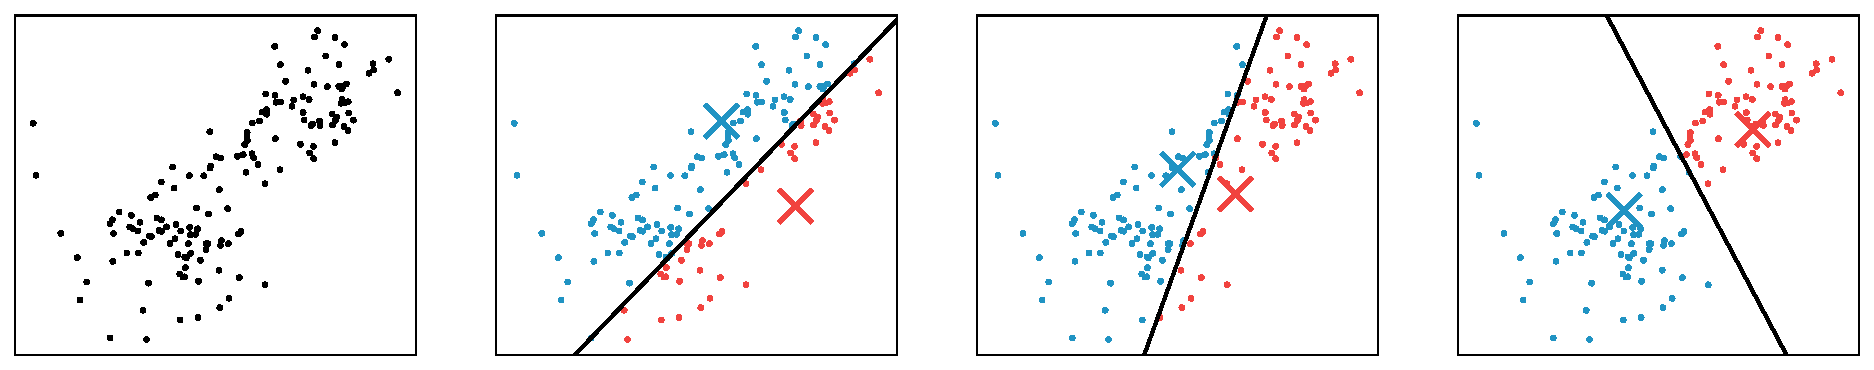
\includegraphics[width=\textwidth]{figures/kmeans.pdf}
    \caption{A figure showing the convergence process of k-means after three iterations.}
    \label{fig:kmeans}
\end{figure}

The k-means algorithm is initialized with $k$ random cluster centers. Then, it minimizes \autoref{eq:kmeans_obj} with a two-step iterative approach. In the first step, the objective function is minimized with respect to $r_{il}$ keeping $\boldsymbol{\mu}_l$ constant:
\begin{equation}
\label{eqn:step2a}
r_{il} = 
    \begin{cases} 
      1 & \text{if } l = \underset{j}{\arg \min}{\|\mathbf{x}_i - \boldsymbol{\mu}_j\|}^2\\
      0 & \text{otherwise}.
   \end{cases}
\end{equation}
\autoref{eqn:step2a} simply states that each data point $\mathbf{x}_i$ is assigned to the cluster with the closest centroid. The second step is minimizing the objective function with respect to $\boldsymbol{\mu}_l$ while keeping $r_{il}$ constant:
\begin{equation}
\label{eqn:step2b}
\boldsymbol{\mu}_l = \frac{\sum_{i=1}^{n}{r_{il} \mathbf{x}_i}}{\sum_{i=1}^{n}{r_{il}}}
        \mbox{ for } 1\leq l \leq k.
\end{equation}
For each cluster, the algorithm computes the new cluster's centroid by using the mean of the cluster's data points. 

\subsection{Limitations}\label{subsection:k-means_limitations}

One of the main shortcomings of the k-means algorithm is that it is sensitive to the initial cluster center placements. As a result, the algorithm may converge to a local optimum instead of a global one. To overcome this problem, the algorithm is usually run multiple times and the best clustering result (i.e.: the one with the lowest within cluster variance) is taken as the final clustering result. Another drawback of the algorithm is that it is parameterized by the cluster number $k$. This is problematic when the dataset is being explored and the number of clusters is unknown.

\subsubsection{Automatically Determining the Cluster Number}

Many clustering algorithms are parameterized by the cluster number $k$. The value of $k$ should be chosen carefully to avoid merging dissimilar clusters (when $k$ is underestimated) or splitting a cluster of similar points (when $k$ is overestimated). In this segment, we outline an automatic hyperparameter search method for choosing $k$.

A good clustering result should yield compact clusters which are well-separated. This translates to clusters having high inter-cluster distances and low intra-cluster variance. The \emph{Silhouette Index} (SI) \parencite{rousseeuw1987silhouettes} is a measure that takes the intra-cluster as well as the inter-cluster distances into account. It is defined as:
\begin{equation}
    SI = \frac{1}{n}\sum_{i=1}^{n}{\frac{\beta(\mathbf{x}_i)-\alpha(\mathbf{x}_i)}{\max\{\alpha(\mathbf{x}_i),\beta(\mathbf{x}_i)\}}}
\end{equation}
where $n$ is the number of data points, $\beta(\mathbf{x}_i)$ is the average distance of $\mathbf{x}_i$ to all points in the nearest cluster and $\alpha(\mathbf{x}_i)$ is the average distance of $\mathbf{x}_i$ to all points in the same cluster. If the clusters are positioned near each other, $\beta(\mathbf{x}_i)$ will be similar to $\alpha(\mathbf{x}_i)$ and the silhouette index scores will be lower for the clustering. On the other hand, clusters which are far away from each other are awarded a higher silhouette score.

The cluster number can be determined automatically from a predefined interval $[k_{min}, k_{\text{max}}]$. This is achieved by running the clustering algorithm for the different values of $k$ in the interval and calculating the SI scores for each clustering result. Finally, the optimal partition is chosen as the one which maximizes SI \parencite{bocking2018determining}.

\section{Image Segmentation}

In the previous section, we discussed clustering a dataset to extract its coherent groups. In this section, we consider extracting clusters in a more specific type of dataset, namely, an image. This is achieved by \emph{segmenting} the image into disjoint non-overlapping regions such that every cluster corresponds to a different real-world object in the image.

The vast literature covering image segmentation includes a variety of methods. However, in this section we focus on two broad categories: color-based segmentation and semantic segmentation.

\subsection{Color-based Segmentation}\label{subsection:color_based_segmentation}

Color-based segmentation methods operate in the color space of an image to generate the final segmentation result. They include thresholding methods, sliding window methods, graph-based methods and clustering-based methods \parencite{dhanachandra2017survey}:

\begin{itemize}
    \item Thresholding techniques divide the pixels of an image into foreground and background pixels based on a threshold hyperparamter. Pixels with intensities greater (lower) than the threshold are classified as being part of the foreground (background). Algorithms with a single global threshold value can sometimes yield poor results since the lightness/intensities in an image can vary greatly. In order to overcome this problem, adaptive thresholding methods divide the image into disjoint crops and threshold each crop independently \parencite{bradley2007adaptive}.
    \item Sliding window approaches inspect the local homogeneity of each pixel by sliding a window of fixed size across the image. Each pixel is then classified as a boundary or non-boundary pixel. Afterwards, region growing is performed around non-boundary pixels to obtain the final segmentation. Examples of such methods are J-image segmentation \parencite{deng2001unsupervised}  and H-segmentation \parencite{jing2003unsupervised}.
    \item Graph-based techniques such as the Felzenszwalb algorithm \parencite{felzenszwalb2004efficient} view the pixels of an image as a set of vertices. These algorithms attempt to construct connected components based on the weighted edges between the vertices. Each connected component formed corresponds to a region in the segmented image.
    \item Clustering-based segmentation methods view the pixels of a color image as data points in the three dimensional color space. Such algorithms attempt to group similarly colored pixels together to generate the final segmentation result.
\end{itemize}

The advantage of the above methods lies in their simplicity since they rely on the basic notion of color. However, since they operate directly on the pixels of the image, they are usually time-consuming and sensitive to pixel-level variation in intensity or illumination. As a result, images containing non-smooth textures are usually poorly segmented.

\subsubsection{Superpixel Algorithms}

In order to address the aforementioned drawbacks associated with processing pixels directly, some approaches introduce an additional preprocessing step. Superpixel-based clustering algorithms perform an image simplification step by inspecting the spatial and color information of the image's pixels. Similarly colored pixels in close vicinity of each other are then grouped together to form \emph{superpixels}. Afterwards, the superpixels are clustered in the color space to yield the final segmentation result (see \autoref{fig:sp_based_clustering_process}). This approach is faster than pixel-based clustering approaches as the clustering is performed on a smaller number of superpixels as opposed to a much greater number of pixels \parencite{stutz2018superpixels}. Additionally, non-uniform pixel intensity is no longer an issue since each superpixel has a homogeneous color which summarizes the colors of the pixels in that superpixel. A good superpixel algorithm should yield compact superpixels which adhere well to boundaries \parencite{jia2014fast}. Moreover, the algorithm should be parameterized by the number of superpixels \parencite{stutz2018superpixels}.

\begin{figure}[htbp]
     \centering
     \begin{subfigure}[b]{0.3\textwidth}
         \centering
         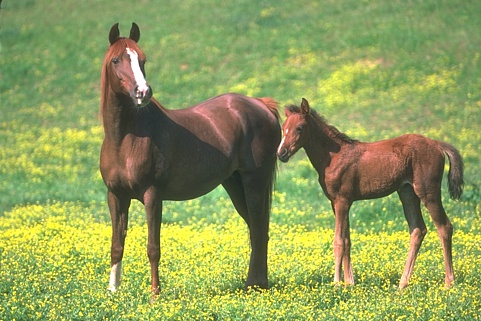
\includegraphics[width=\textwidth]{figures/horses.jpg}
         \caption{Original image}
     \end{subfigure}
     \hfill
     \begin{subfigure}[b]{0.3\textwidth}
         \centering
         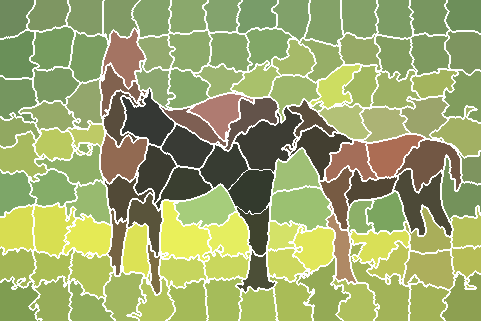
\includegraphics[width=\textwidth]{figures/contours_horses.png}
         \caption{Superpixel image}
     \end{subfigure}
     \hfill
     \begin{subfigure}[b]{0.3\textwidth}
         \centering
         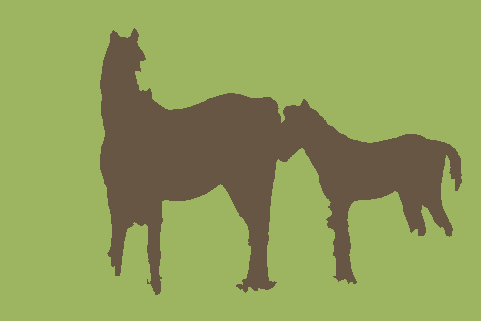
\includegraphics[width=\textwidth]{figures/clustered_horses.png}
         \caption{Final segmentation}
     \end{subfigure}
    \caption{An outline of the superpixel-based clustering process. The original image (a) is transformed into a superpixel image (b). The final segmentation (c) is obtained by clustering similar superpixels together.}
    \label{fig:sp_based_clustering_process}
\end{figure}

Superpixel algorithms can be classified into various categories including watershed-based, graph-based and clustering-based algorithms \parencite{stutz2018superpixels}. Clustering-based algorithms such as Simple Linear Iterative Clustering (SLIC) \parencite{achanta2010slic} evolve from partitioning algorithms like k-means. They attempt to group similar pixels into superpixels based on spatial proximity and color similarity. Compared to other superpixel algorithms, clustering-based superpixel algorithms are fast and can be easily extended to multi-dimensional images.

\subsubsection{Fuzzy Simple Linear Iterative Clustering}

The SLIC algorithm \parencite{achanta2012slic} operates in a similar way to k-means. Like many other superpixel algorithms, SLIC is typically applied to color images in the CIELAB color space, which is perceptually uniform for small color differences. The algorithm defines each pixel as a five dimensional vector comprised of two spatial coordinates and three color coordinates.

SLIC takes an initial superpixel number $K$ as input. The algorithm starts by sampling $K$ cluster centers placed on a regular grid. The grid interval length is defined as $S=\sqrt{{N}/{K}}$ where $N$ is the number of pixels in the image.
Afterwards, each cluster employs a local search method when searching for possible members (as opposed to the global search employed by k-means). The cluster considers only those points which are within a $2S \times 2S$ fixed window search region around the cluster's center.

The employment of a local instead of a global search is due to the fact that neighboring pixels are highly correlated and are much more likely to belong to the same object than pixels which are far away from each other \parencite{achanta2012slic}. Moreover, the local search speeds up the algorithm's run time by limiting the search region for each cluster. SLIC then proceeds to relocate pixels to their closest superpixels and update the superpixel centers until a maximum number of iterations is reached. It is important to note that the final cluster number can fall below the initial value of $K$. This is due to some of the clusters losing all of their members to other clusters during the relocation process.

The SLIC distance function plays a vital role in determining the final shape of the superpixels. Instead of calculating the Euclidean distance between a point and a cluster center in the 5D space, the SLIC distance function balances pixel proximity and color similarity. Additionally, it offers control over the compactness of the superpixels. According to SLIC, the distance between point $\mathbf{x}_i$ and cluster center $\mathbf{c}_j$ is defined as follows \parencite{achanta2010slic}:
\begin{equation}
    d(\mathbf{x}_i, \mathbf{c}_j) = \sqrt{\sum_{l=1}^{L}{(f_i^{(l)} - f_j^{(l)})^2}} + \frac{m}{S}\sqrt{(x_i-x_j)^2 + (y_i-y_j)^2}
    \label{eq:slic}
\end{equation}
where $L$ is the number of channels in the image, $f^{(l)}$ is the $l$-th color channel, $m$ is a compactness coefficient used to control the shape of the superpixels and $x$ and $y$ represent the horizontal and vertical spatial coordinates, respectively. The first summand in the above equation calculates the color space dissimilarity while the second summand calculates the spatial distance (normalized by the grid size and weighted by $m$). The value of $m$ controls the balance between the color and spatial dissimilarity. A greater value of $m$ weights the spatial distance more than the color space distance. This results in more compact superpixels. \autoref{fig:slic_m} shows the effect of increasing $m$ on the final superpixel shapes. By looking at the figure, it is clear that a larger value of $m$ results in more tightly packed and square shaped superpixels.

\begin{figure}[t]
     \centering
     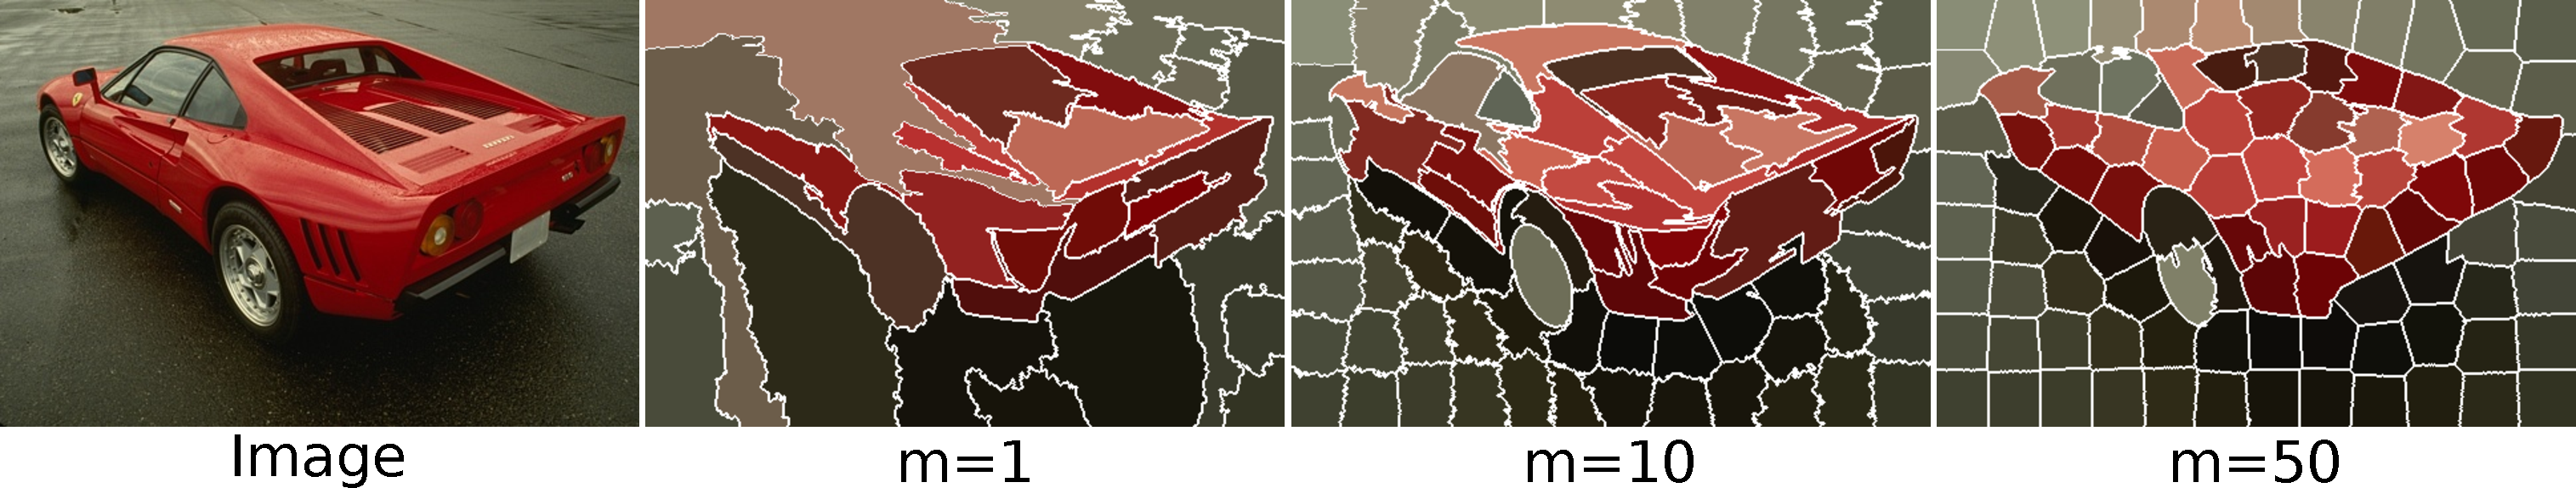
\includegraphics[width=\textwidth]{figures/slic_m.pdf}
    \caption{SLIC superpixels for different values of $m$ (see \autoref{eq:slic}).}
    \label{fig:slic_m}
\end{figure}

Fuzzy SLIC (FSLIC) \parencite{wu2020fuzzy} extends SLIC by softening the memberships of the points to the clusters such that the memberships can take on values between $0$ and $1$. Furthermore, FSLIC reinforces each pixel's membership to a cluster by the pixel's neighborhood's membership to that cluster. The original membership of a point $\mathbf{x}_i$ to cluster $\mathbf{c}_j$ is defined as \parencite{wu2020fuzzy}:
\begin{equation}
    u_{ij} = \left( \sum^{s_i}_{k=1}{\left(\frac{d(\mathbf{x}_i, \mathbf{c}_j)}{d(\mathbf{x}_i, \mathbf{c}_k)}\right)^{\frac{2}{t-1}} } \right)^{-1}
\end{equation}
where $t$ is the fuzziness coefficient, $s_i$ is the number of clusters which contain point $\mathbf{x}_i$ in their grid search region and $d(\mathbf{x}_i, \mathbf{c}_j)$ is the SLIC distance function between point $\mathbf{x}_i$ and center $\mathbf{c}_j$ (see \autoref{eq:slic}).

Afterwards, the pixel's neighborhood's membership is calculated as follows:
\begin{equation}
    h_{ij} = \sum_{p \in \mathcal{N}_i}{u_{pj}}
\end{equation}
where $\mathcal{N}_i$ is the small square neighborhood defined around pixel $\mathbf{x}_i$. Finally, a pixel's reinforced membership combines its original membership with its neighborhood's membership:
\begin{equation}
    u'_{ij} = \frac{u_{ij}^{f}h_{ij}^{g}}{\sum_{k=1}^{s_i}{u_{ik}^{f}h_{ik}^{g}}}
\label{eq:fslic_memberships}
\end{equation}
where $f$ and $g$ are control hyperparameters used to weight the effect of $u_{ij}$ relative to $h_{ij}$. In a homogeneous region, the neighborhood's membership either strengthens the original membership of a non-noisy pixel or corrects the membership of a noisy pixel. As a result, FSLIC is robust to multiple different types of noise and can adhere well to boundaries \parencite{wu2019improved}.

\begin{figure}[t]
    \centering
    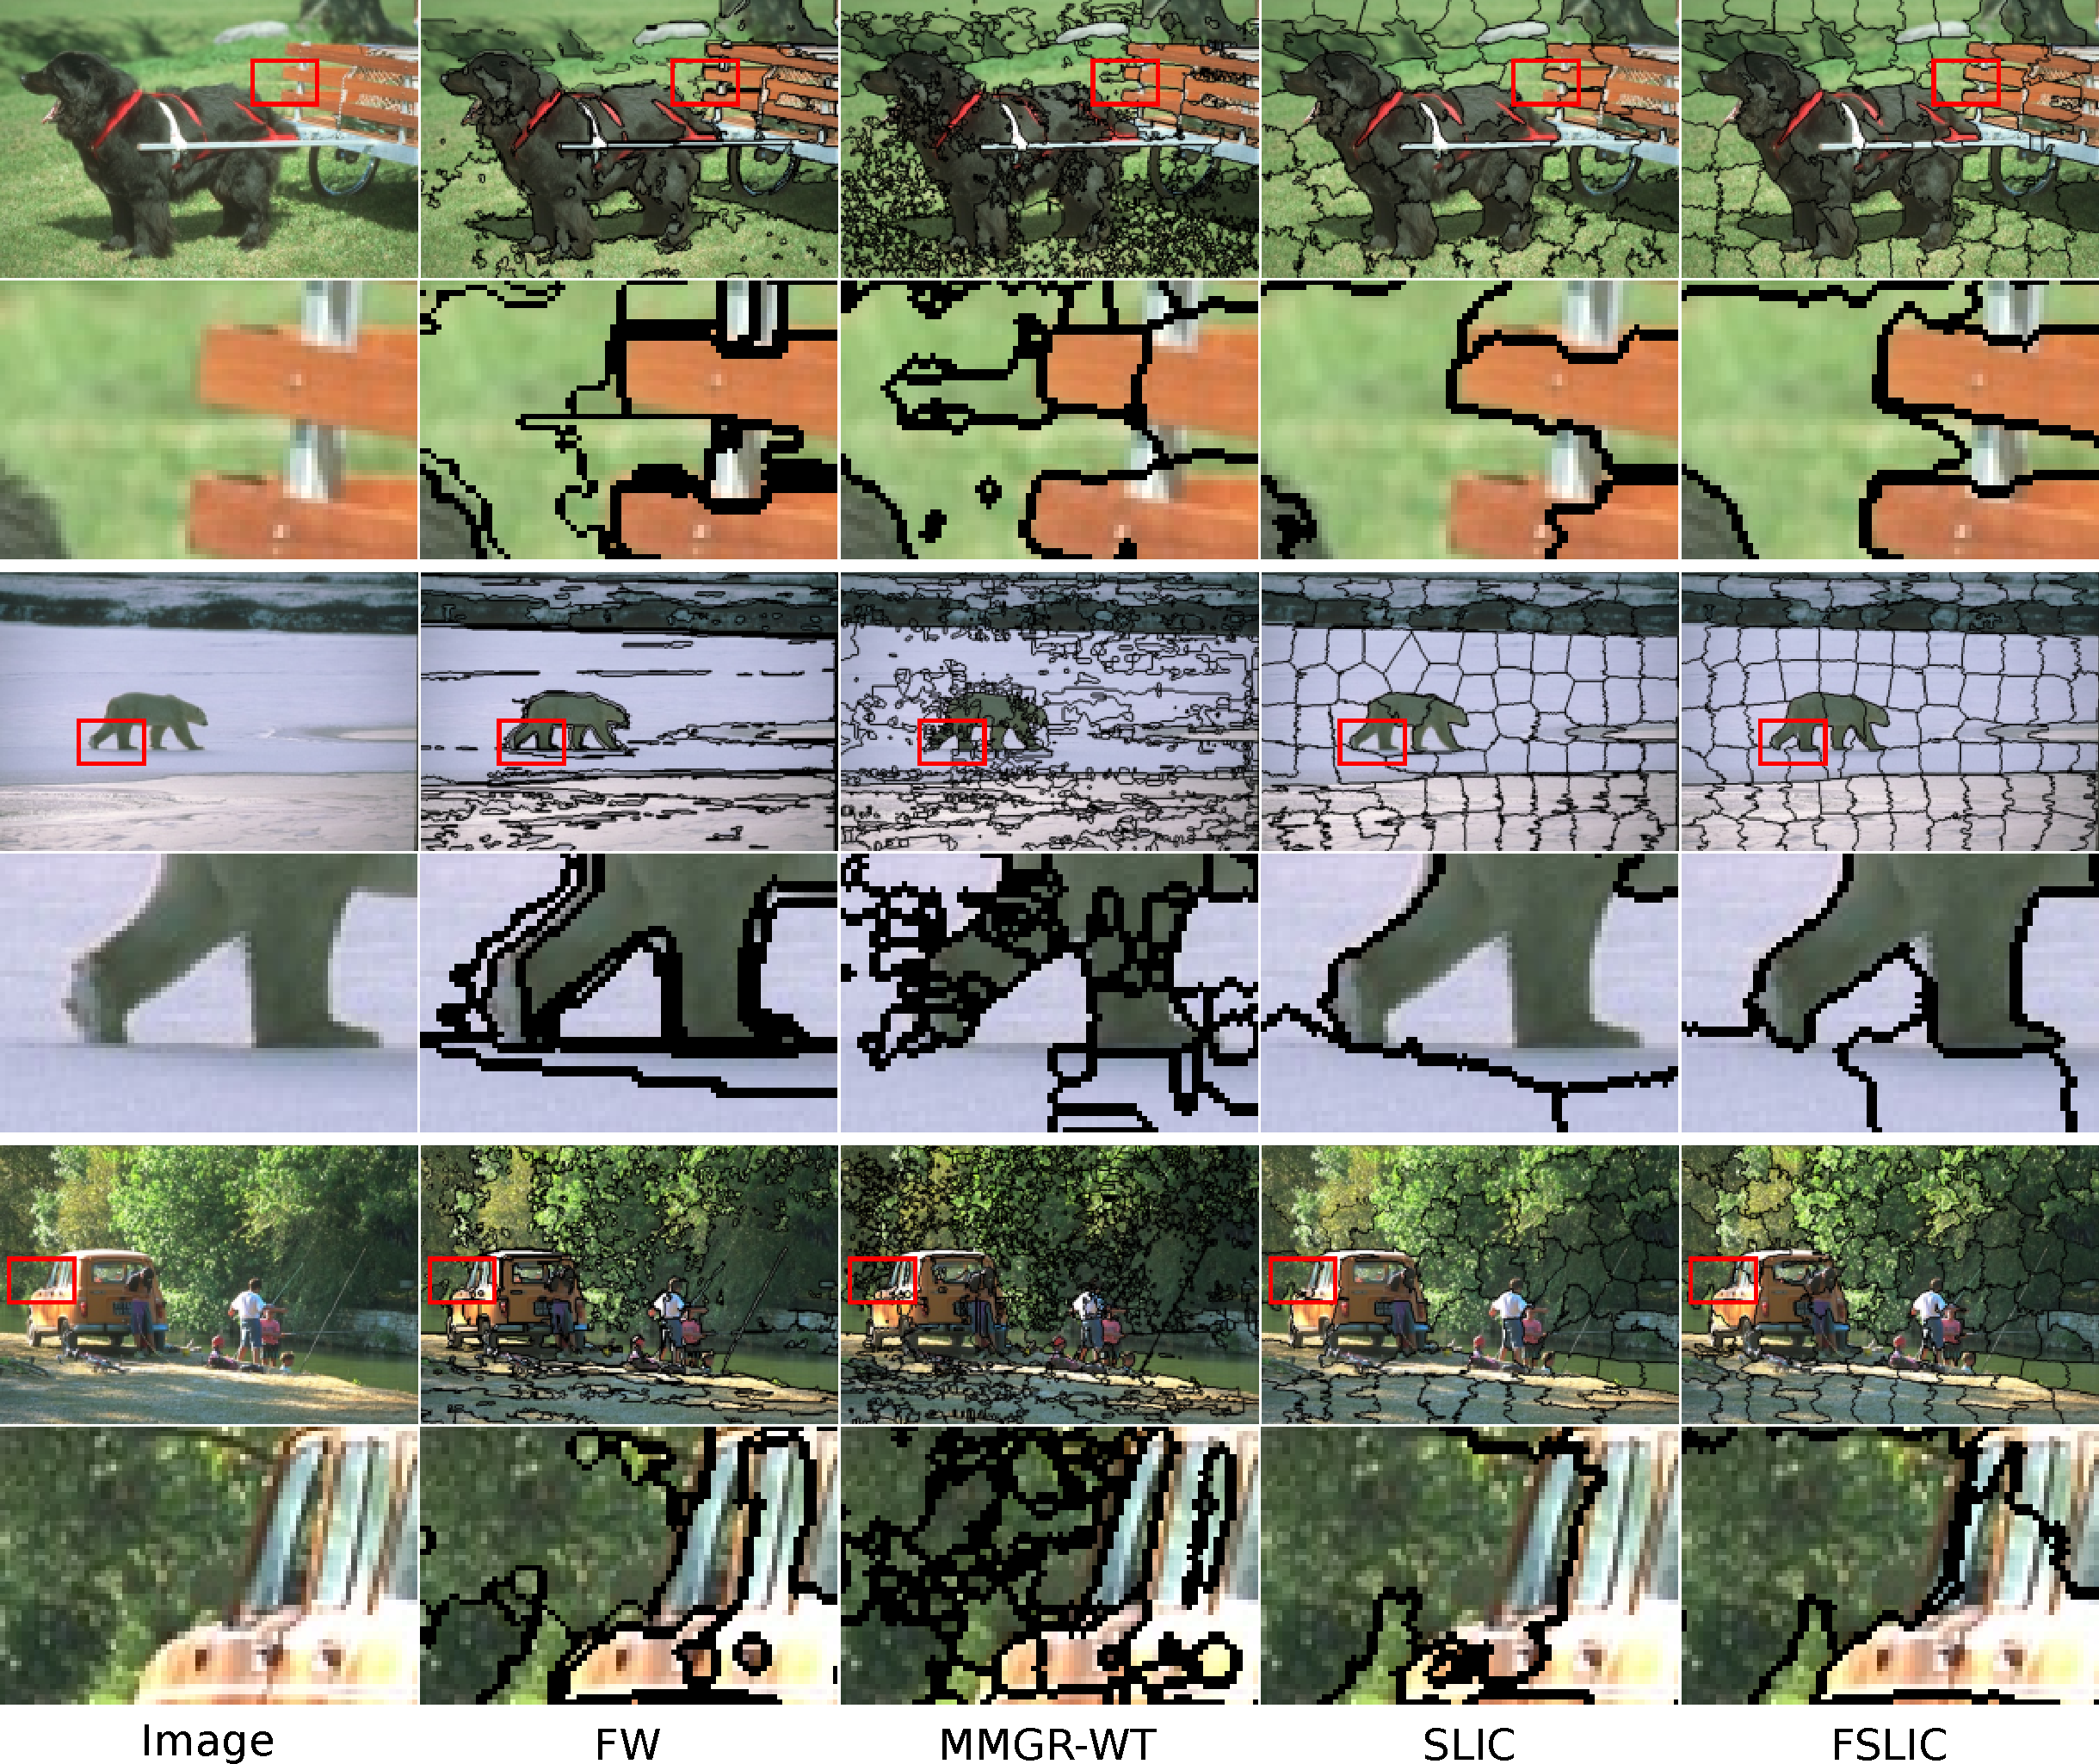
\includegraphics[width=\textwidth]{figures/superpixel_comparison.pdf}
    \caption{A figure showing the superpixel segmentations obtained from four different algorithms on several images.}
    \label{fig:superpixel_comparison}
\end{figure}

\autoref{fig:superpixel_comparison} shows the superpixel results obtained using SLIC, FSLIC, the Felzenszwalb algorithm (FW) and the watershed transform with multi-scale morphological gradient reconstruction (MMGR-WT) \parencite{lei2018superpixel}. The four algorithms were initialized with their default parameters. The figure clearly shows that FSLIC can generate regularly shaped superpixels that have a stronger adherence to object boundaries.


\subsubsection{Superpixel-based Fuzzy C-means}

The final step in a superpixel-based segmentation approach is to cluster similarly colored superpixels together. Clustering the superpixels directly with a partitioning algorithm such as fuzzy c-means might not always yield the best results. This is because the superpixel sizes are not taken into account. Larger superpixels should affect the clustering more than smaller superpixels. Superpixel-based fuzzy c-means (SFCM) incorporates the superpixel sizes into its objective function to overcome this problem. Its objective function is defined as \parencite{lei2018superpixel}:
\begin{equation}
    J = \sum_{l=1}^{k}{\sum_{i=1}^{q}{S_i u_{il}^t \left\| \frac{\sum_{\mathbf{x} \in R_i}{\mathbf{x}}}{S_i} - \boldsymbol{\mu}_l \right\| ^2}}
\label{eq:obj}
\end{equation}
where $q$ is the number of regions (superpixels), $k$ is the number of clusters, $u_{il} \in (0, 1)$ is the soft membership of region $i$ to cluster $l$, $t$ is the fuzziness coefficient used to control the memberships, $R_i$ is the $i$-th superpixel, $S_i$ is the number of pixels in $R_i$ and $\boldsymbol{\mu}_l$ is the center of cluster $l$. By minimizing \autoref{eq:obj} with respect to the different unknown variables, we obtain equations for the calculation of the memberships and the cluster centers. The algorithm then proceeds by relocating superpixels between clusters until there is no significant change in the soft memberships. Finally, each superpixel is assigned to the cluster to which it has the maximum membership. 

\begin{figure}[t]
    \centering
    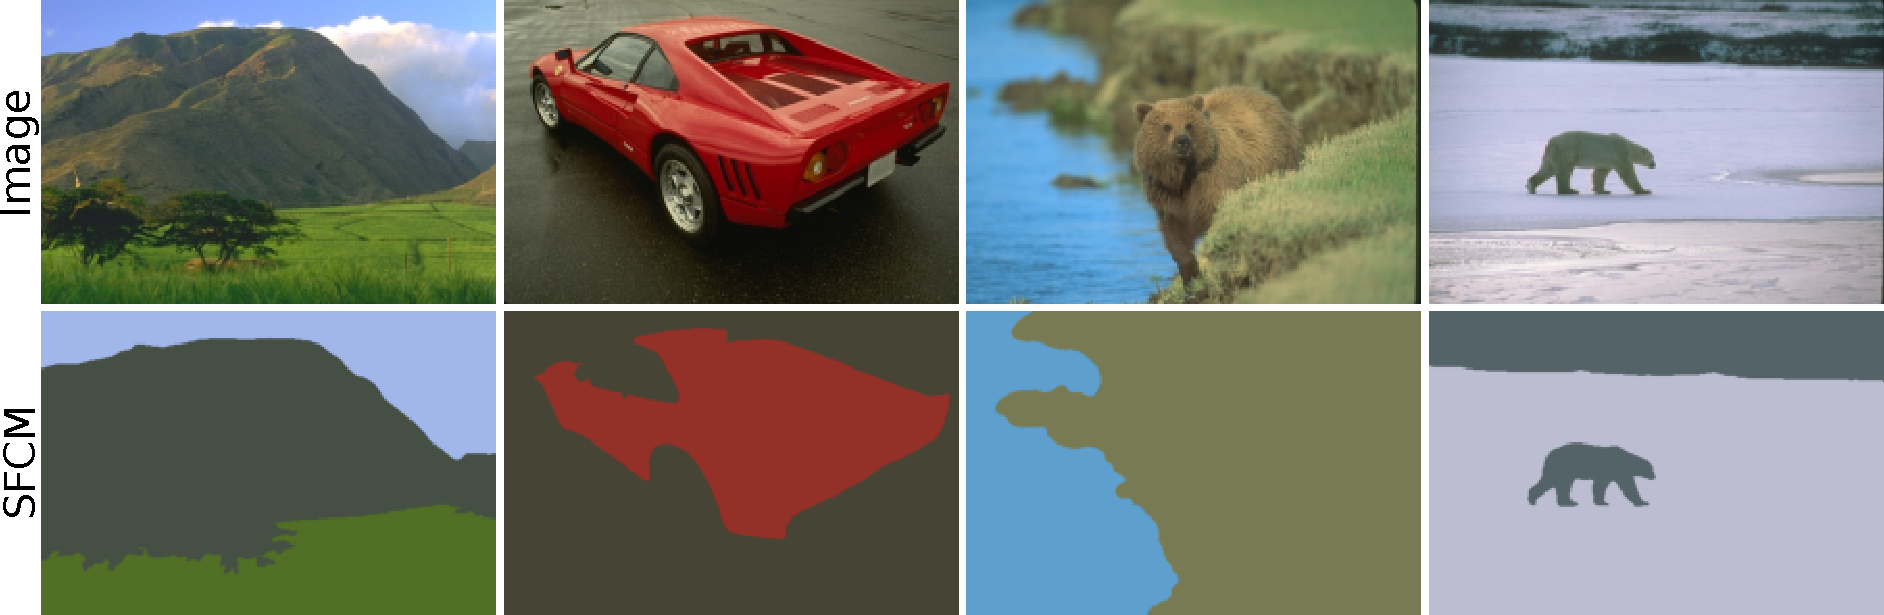
\includegraphics[width=\linewidth]{figures/clustered_images.pdf}
    \caption{Four images from BSD500 (top row) and their corresponding segmentation results which were generated using FSLIC followed by SFCM (bottom row). The number of clusters is chosen according to the scatter plot of the superpixels in color space.}
    \label{fig:sffcm}
\end{figure}

\subsubsection{Limitations}

\autoref{fig:sffcm} shows the results of clustering FSLIC superpixels using SFCM. The results show that the superpixel-based clustering approach is more suitable for segmenting images with a significant color contrast between the different objects in the image. However, images with similarly colored objects are poorly segmented. The algorithm interprets the different objects as being similar and assigns them to the same cluster (third and fourth column of \autoref{fig:sffcm}).

\subsection{Semantic Segmentation}

The previous subsection showed that algorithms which only rely on pixel colors fail at separating similarly colored objects in the image. This motivates the usage of statistically trained machine learning models that can extract semantic information from the image. In the past decade, deep learning approaches have been widely used in imaging tasks such as classification and semantic segmentation. Semantic segmentation refers to assigning pixel-wise class labels to the pixels of an image \parencite{minaee2021image}. The final image can be thought of as a map or a function from pixel spatial coordinates to class labels. In this subsection, we give a brief introduction to deep learning using neural networks before reviewing traditional semantic segmentation architectures. Afterwards, we discuss the limitations associated with semantic segmentation in general.

\subsubsection{Neural Networks and Learning}

The primary deep learning model is the neural network (also known as the multi-layer perceptron) \parencite{goodfellow2016deep}. It is made up of neurons, which are the main building blocks of any deep learning model. The neurons of the network are usually arranged in layers, where the first and final layers are referred to as the input and output layers, respectively. The layers in between are known as the hidden layers of the network. The inputs to the neurons in one layer are the outputs of the neurons in the preceding layer. \autoref{fig:nn} shows a typical neural neural network architecture.
\vspace{2 mm}
\begin{figure}[thbp]
    \centering
    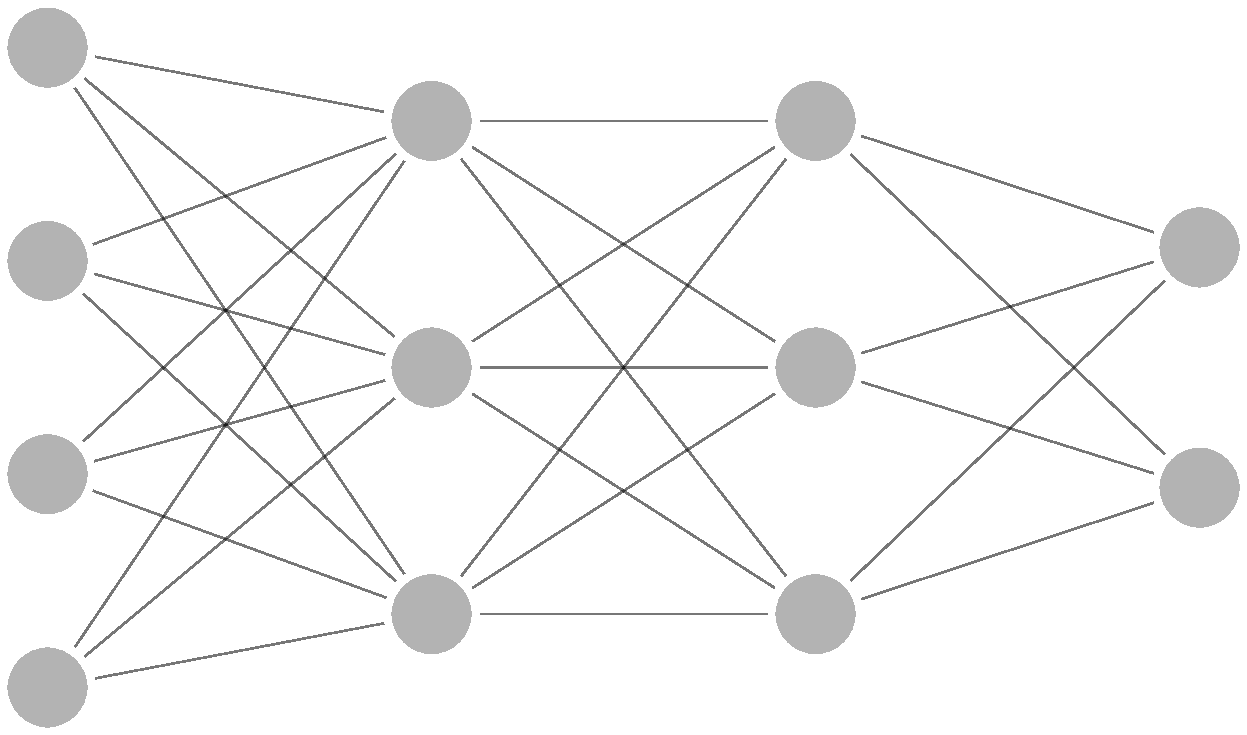
\includegraphics[width=.5\linewidth]{figures/nn2.pdf}
    \caption{A neural network with two hidden layers. Aside from the input layer, each layer's neurons receive their inputs from the previous layer.}
    \label{fig:nn}
\end{figure}

Each neuron in the network holds a value known as the neuron's activation. A neuron's activation is calculated as the weighted sum of its input activations plus a bias term. In other words, each neuron calculates a simple linear transformation of its input. Since the composition of linear transformations is also linear, two successive hidden layers applying linear transformations to their inputs can be compressed into one layer. Therefore, each linear transformation is usually followed by the element-wise application of a non-linear function. This introduces non-linearity in the network, allowing it to act as a universal function approximator. A common non-linear activation function is the Rectified Linear Activation Unit (ReLU) which is defined as $\text{ReLU}(u^{(l)}) = \max\{ 0, u^{(l)}\}$
for each neuron $u$ in layer $l$.

The entire neural network can be thought of as a non-linear transformation of the input into the output. Depending on the application domain, the output of the network can have many interpretations. For example, an output layer of size $k$ can be interpreted as a classification of the input into one of $k$ categories.

In order to generate a meaningful output, the parameters (weights and biases) of the network have to be optimized. This is done by training the network on a set of training data consisting of input-output pairs. The network is trained to match the predicted output against the known output so that it can adjust its parameters accordingly. This process is known as the learning or training phase of the network.

Neural networks are typically trained through loss minimization. That is, after the input from the training data is propagated through the network, a loss function which compares the predicted output against the known output is minimized with respect to the network's parameters. The choice of the loss function often depends on the learning task. For instance, the mean squared error is often used for regression tasks while the cross-entropy loss function is typically used for classification tasks \parencite{nielsen2015neural}.

\subsubsection{Convolutional Neural Networks}


Standard neural networks are inefficient when working with very high-dimensional data, such as images. This is due to the number of parameters scaling linearly with the input dimensionality, and models with more parameters need more data to train.
Convolutional neural networks (CNNs) are a special type of neural network that are commonly used for imaging tasks. The number of parameters in CNNs does not depend on the input's dimensionality since they utilize a special operator known as the \emph{convolution} operator.

\begin{figure}[thbp]
    \centering
    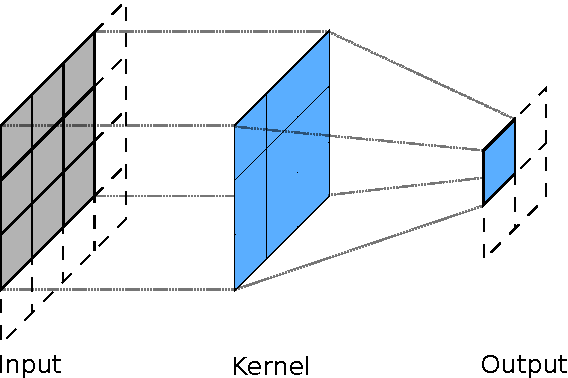
\includegraphics[width=.5\textwidth]{figures/conv4.pdf}
    \caption{Discrete 2D convolution.}
    \label{fig:conv}
\end{figure}

The convolution operator can capture local information in a given image. It is typically used to extract features at different locations in an image by sliding a small window function, known as the \emph{kernel}, around the image (see \autoref{fig:conv}). Since images are defined in a discrete input space, we will focus on the discrete convolution operator. The discrete convolution operator in 2-D (usually denoted by an asterisk) is defined as\footnote{The actual operator shown is the cross-correlation operator. True convolution would require flipping the kernel (by replacing the pluses with minuses in the function arguments) to maintain the commutativity property. However, we follow the literature by defining convolutions without kernel flipping.}:
\begin{equation}
    (I * K)(i, j) = \sum^{}_{r}{\sum^{}_{s}{I(i+r, j+s) \times K(r, s)}}
\end{equation}
where $I$ is the image function of a single channel image defined in the pixel space and $K$ is a small kernel matrix. The local variables $r$ and $s$ are used to access the different entries in the kernel matrix.

Different kernels can extract different features in an image. The relative difference between the kernel entries controls the desired effect on the output image. The size of the kernel controls the scale of the features to be extracted. A small (large) kernel can be used to capture local (global) context in the image.
\autoref{fig:edges} shows the result of convolving an image with different kernels to detect different types of edges in the image.

\begin{figure}[thbp]
    \centering
    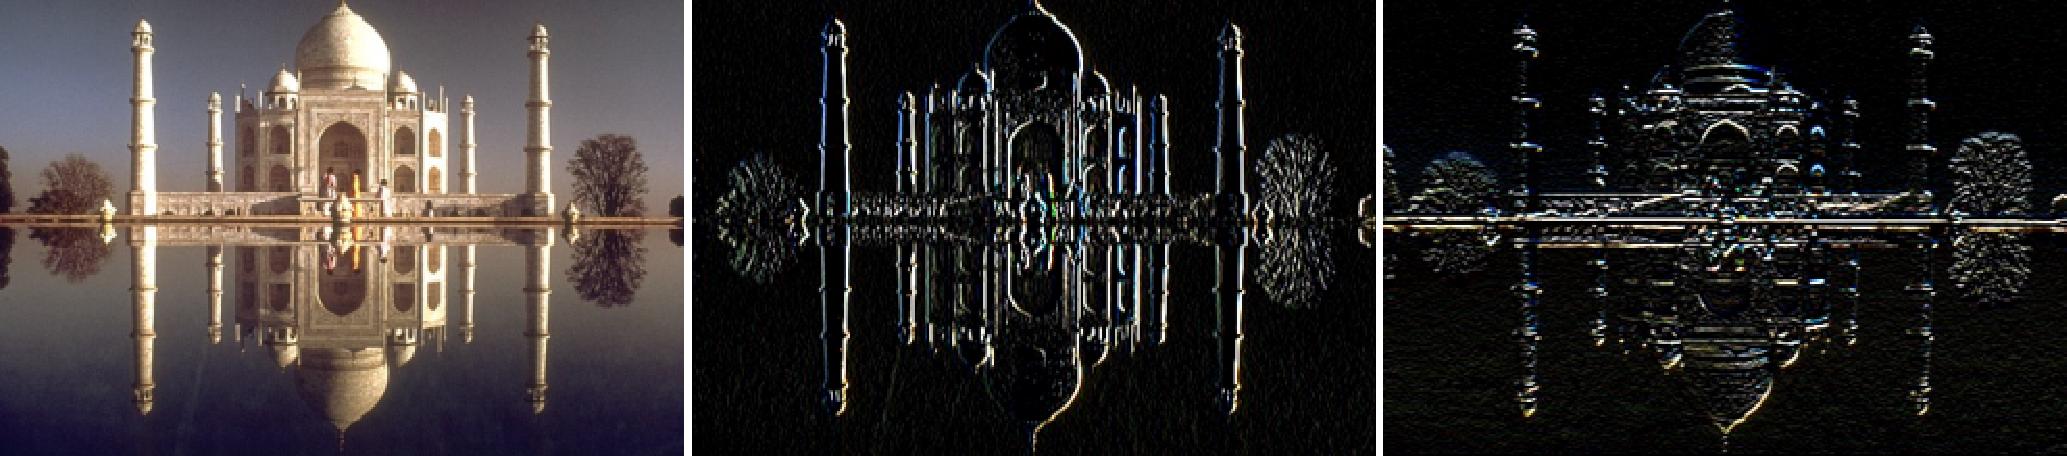
\includegraphics[width=\textwidth]{figures/sobel.pdf}
    \caption{The original image (left) has been convolved with two different kernels to detect vertical edges (middle) and horizontal edges (right).}
    \label{fig:edges}
\end{figure}

Nowadays, imaging tasks such as classification are approached by using CNNs which apply various convolutions to images. A CNN is typically made up of two parts: a feature extractor and a classifier. Just like an MLP, the feature extractor of a CNN is arranged in layers of neurons, where each layer can be visualized as a 3D tensor of neurons. There are 3 main types of layers in the feature extractor:
\begin{enumerate}
    \item The convolutional layer convolves its input with multiple kernels in order to extract multiple features from its input tensor. Using convolutions in neural networks also facilitates memory efficiency through parameter sharing \parencite{goodfellow2016deep}. In a standard MLP, each weight and bias in one layer is used only once. However, in (the feature extractor of) a CNN, the same set of weights (defined in the kernel) is shared by all the neurons.
    \item Activation layers typically follow convolutional layers \parencite{hesamian2019deep}. The activation layer applies a non-linear activation function such as the ReLU function to every neuron in the layer.
    \item The final type of layer is known as the pooling layer. Pooling is an operation that provides a compact representation of the layer's input. It is able to summarize the activations in the neighbourhood of a particular neuron. For example, the \emph{max pooling} operator replaces each block of activations in the input tensor with the maximum activation in that block. Pooling is often used to decrease the resolution of the input tensor. This is known as downsampling the input. The subsequent layers often add more channels to their input tensor to compensate for the reduced spatial resolution.
\end{enumerate}

The feature extractor is typically followed by a classifier, which is a fully connected MLP that categorizes its input into one of many categories. The feature maps (3D tensor) output by the feature extractor are fed into the classifier. The final layer of most classifiers is a softmax activation layer. The softmax function is used to normalize the final layer's activations so that they can be interpreted as probability scores. After applying the softmax function to a layer, the activations of the layer sum up to 1 and each neuron's activation lies in the $(0,1)$ interval. Together the feature extractor and the classifier form the CNN, which can be trained on a training dataset in a similar fashion to a standard MLP.

\subsubsection{Pixel-wise Classification}

As mentioned in the beginning of this subsection, the task of semantic segmentation is to assign a class label to every pixel in the image. Several CNN architectures have been proposed in the literature for this purpose. A review on popular semantic segmentation architectures can be found in \textcite{taghanaki2021deep}.

One of the first CNN architectures designed for semantic segmentation was the fully convolutional network (FCN) \parencite{long2015fully}. FCN consists of an encoder (feature extractor) module made up of convolutional, activation and pooling layers to capture the semantic information in the image. In other words, FCN does not have a classifier module. The final layer in FCN uses deconvolution to output a feature tensor of the same spatial resolution as the input image. Each pixel in the output tensor is a vector of class prediction scores. Finally, the segmentation map is obtained by assigning each pixel to its most likely class label. Several architectural improvements have been made to the original FCN in order to increase its segmentation accuracy. U-net \parencite{ronneberger2015u} proposed to extend the original FCN by introducing a decoder module after the encoder. The decoder would gradually upsample the deep features output by the encoder while simultaneously reusing shallow features from the encoder to preserve object boundary details. Pyramid scene parsing network (PSPNet) \parencite{zhao2017pyramid} was proposed to capture different levels of detail in the image. PSPNet uses a pyramid pooling module to extract multi-scale features, thereby capturing both local and global context information in the image. DeepLabv3+ \parencite{chen2018encoder} combined encoder-decoder style with a special pyramid pooling module to capture multi-scale features as well as preserve location information. The architecture was able to achieve state-of-the-art performance on multiple datasets.

\subsubsection{Limitations}

\begin{figure}[t]
    \centering
    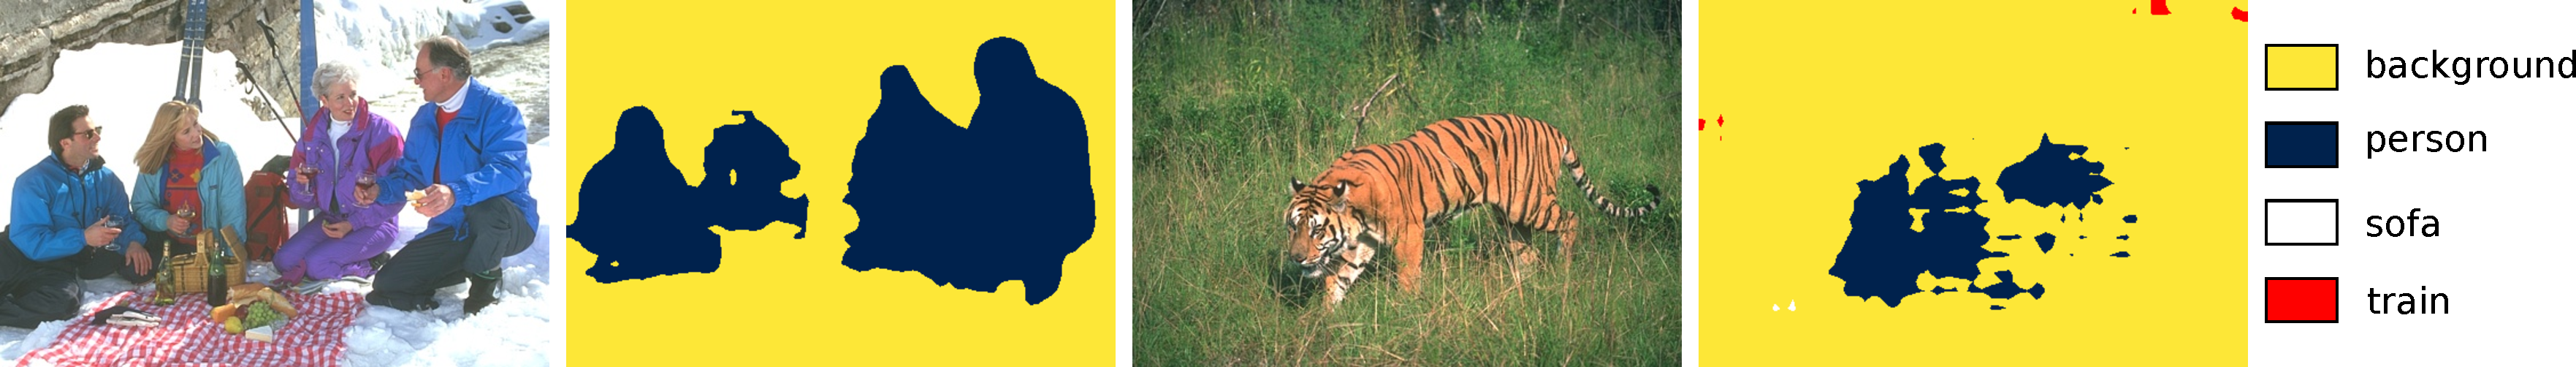
\includegraphics[width=\textwidth]{figures/semantic.pdf}
    \caption{Two images segmented using PyTorch's pretrained fcn\_resnet101 \parencite{paszke2019pytorch}.}
    \label{fig:semantic_segmentation}
\end{figure}

One major drawback of semantic segmentation is its restricted application domain. Due to the limited choice of labels that semantic segmentation models can assign to the pixels of an image, the models cannot be used to segment all types of images. \autoref{fig:semantic_segmentation} shows the results obtained using an FCN to segment two images. The first image seems to be properly segmented since it contains objects that the model has seen during training. By comparison, the second image of the tiger is poorly segmented since the model has not been trained on the types of objects in the image. 

Another issue with semantic segmentation is the need for labelled data to train a model. However, this is not possible in situations where we wish to explore the different objects present in an image and hence, cannot use labelled data to train a CNN. Also, obtaining labelled data for semantic segmentation can be very time-consuming, as every pixel in every image has to be manually labelled \parencite{chen2019unsupervised}.

\subsection{Unsupervised Object Segmentation}

In order to address some of the limitations of color-based and semantic segmentation methods, a different set of unsupervised approaches have been proposed in the literature. These approaches do not suffer from the dependency on a limited set of class labels while still visiting the feature space of a deep learning model to interpret the image.

\textcite{kanezaki2018unsupervised} performed unsupervised segmentation by optimizing a CNN end-to-end style. The network's output segmentation mask had to enforce a set of spatial and feature similarity constraints. Finally, the refined output was used to optimize the network's layers through backpropagation. \textcite{chen2019unsupervised} explored segmentation via object redrawing by using a complex architecture based on a generative adversarial network (GAN). The core idea was to extract object masks and subsequently use the GAN to generate an object in that mask. Then, all the generated objects would be assembled together according to their masks to yield the final segmentation. \textcite{van2021unsupervised} trained a network in an unsupervised setting by employing contrastive learning. The network was trained to generate similar pixel embeddings for similar objects and dissimilar embeddings for dissimilar objects. The final segmentation mask was obtained by clustering the network's learned pixel embeddings.

\textcite{guerin2018unsupervised} explored unsupervised object classification by means of transfer learning. Feature tensors of multiple images were extracted from a pretrained CNN and clustered into coherent groups to identify similar images.
In our work, we adopt a similar idea to extract objects from an image. Instead of clustering the feature tensors of multiple images, we cluster the pixel-wise feature representations of a single tensor to exploit the spatial coherence of the pixels in the image and extract the different objects found in it. Unlike some of the methods mentioned in the previous paragraph, the parameters of the network are not further fine-tuned.